\scanpage{73}
\deleted{
\uline{Choisissons} \inserted{\uline{\unsure{loc (Zar)}}} section $s_0$ de $X$ admissible pour le syst. des $(\tau_i^X)$,
(déterminé mod homothétie dans $\overline E=X\setminus C$ muni de \uline{l'origine $c$}).

Cas $c\notin C$ en tt pt \inserted{i.e. $\rho$ inv}
($n$ impair et $\rho'$ \deleted{\unsure{iff}} inv., ou
$n$ pair \deleted{et $2$ inv} \inserted{(car $\rho=2\rho'$)})
--- \deleted{donc est} Donc on est dans les conditions suivantes
(identifions $\overline E$ à $V$ grâce à l'origine $c=0$)

a) $\varphi_G^V:G\longrightarrow
\deleted{\unsure{\operatorname{Aut}(V),\mathbf G_m}}O(f)$

b) \deleted{Section $s_0$ d} base $s_0$ de
$D_0^*=\bigcap_{1\leq i\leq n}H_i^!$
$(H_i^!=H_i\setminus H_i\cap\unsure{\overline C|C})$
}
\margin{$\unsure{a_{-1}^*}$}

On a $\boxed{\text{dans }\check V}$
\[
\begin{aligned}
a_0^\vee&=\deleted{\lambda_0-1}(\lambda_0-1)a_0^*+\beta_0a_1^*\\
a_i^\vee&=a_{i-1}^*+(\lambda_i-1)a_i^*+\beta_i a_{i+1}^*
&&1\leq i\leq n-1\\
a_n^\vee&=a_{n-1}^*+(\lambda_n-1)a_n^*
\end{aligned}
\]
\margin{\uline{NB} $\rho$ inv. \unsure{exprime} ici que, \unsure{posant}
$D_0=\bigcap_{1\leq i\leq n}H_i$,
i.e. $a_0^\vee|D_0\neq0$ sur chaque fibre
(conséquence des \unsure{deuxièmes condit$^\circ$s} dans $1^\circ$)}
\deleted{\unsure{b)\quad s_0\quad a_{-1}}}

(Attention au chgt des notations, il n'y a plus de
$a_{-1},a_{-1}^*\ \cdots$)
\[
\deleted{\unsure{a_i^\vee}}\quad
\figure{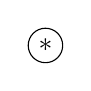
\begin{tikzpicture}[baseline=(s.base)]\node[draw,circle,inner sep=2pt](s){$*$};\end{tikzpicture}}
\qquad
s_0=\deleted{\unsure{\frac{\sigma}{\rho}a_0+\zeta}}
\inserted{=\widetilde s_0=}
-\frac1\rho(\zeta_0a_0+\zeta_1a_1+\mathbin{-}+\zeta_n a_n)
\]
\margin{On suppose pour simplifier maintenant les $\lambda_i=-1$
($\tau_i$ \uline{réflexions})}
\[
\zeta_n=1,\qquad \zeta_{n-1}=2,\qquad
\zeta_i=L_{\unsure{n+i|n-i}}(\beta_{n-1},\ldots,\beta_{i+1})
\]
\[
\left[
\begin{aligned}
\tau_i^V(s_0)&=s_0&&1\leq i\leq n\\
\text{i.e.}\quad\langle s_0,a_i^\vee\rangle&=0&&1\leq i\leq n\\
\tau_0^Vs_0&=s_0+a_0&&\text{i.e.}\quad\langle s_0,a_0^\vee\rangle=1
\end{aligned}
\right]
\]
\[
\unsure{\overline\zeta_0|\zeta_0}
=L_n(\beta_{n-1},\ldots,\beta_1)
=L_n(\beta_1,\mathbin{-},\beta_n)=\sigma
\]

C) Formes quadratiques invariantes :
\deleted{\unsure{constituent}}\inserted{elles forment}
un \deleted{torseur} $\mathcal O_S$-Module \inserted{loc}
libre de rg $1$. On normalise par
\[
\left\{
\begin{aligned}
f_V(a_0)&=1\quad\Rightarrow\quad
f_V(a_i)=\beta_0\beta_1\mathbin{-}\beta_{i-1}\\
\varphi(a_i,a_j)&=\unsure{\{0\}|0}
\quad\text{si }i,j\text{ non consécutifs}\\
\varphi(a_i,a_{i+1})&=-\beta_0\mathbin{-}\beta_i
\end{aligned}\right.
\]
\mspage{72}

